\documentclass{article}
\newcommand{\ve}[1]{\mathbf{#1}}
\newcommand{\dd}{\text{d}}
\newcommand{\ba}{\ve{a}}
\newcommand{\bb}{\ve{b}}
\newcommand{\bA}{\ve{A}}
\newcommand{\bu}{\ve{u}}
\newcommand{\bv}{\ve{v}}
\newcommand{\br}{\ve{r}}
\newcommand{\bt}{\ve{t}}
\newcommand{\bn}{\ve{n}}
\newcommand{\bc}{\ve{c}}
\newcommand{\bq}{\ve{q}}
\newcommand{\bff}{\ve{f}}
\newcommand{\bF}{\ve{F}}
\newcommand{\bx}{\ve{x}}
\newcommand{\hx}{\hat{x}}
\newcommand{\hbx}{\hat{\ve{x}}}
\newcommand{\bS}{\ve{S}}
\newcommand{\bU}{\ve{U}}
\newcommand{\bV}{\ve{V}}
\newcommand{\bQ}{\ve{Q}}
\newcommand{\by}{\ve{y}}
\newcommand{\be}{\ve{e}}
\newcommand{\bs}{\ve{s}}
\newcommand{\bp}{\ve{p}}
\newcommand{\bP}{\ve{P}}
\newcommand{\bR}{\ve{R}}
\newcommand{\bM}{\ve{M}}
\newcommand{\bI}{\ve{I}}
\newcommand{\vq}{\vec{q}}
\newcommand{\balpha}{\boldsymbol{\alpha}}
\newcommand{\bkappa}{\boldsymbol{\kappa}}
\newcommand{\bLambda}{\boldsymbol{\Lambda}}
\newcommand{\blambda}{\boldsymbol{\lambda}}
\newcommand{\bmu}{\boldsymbol{\mu}}
\newcommand{\bOmega}{\boldsymbol{\Omega}}
\newcommand{\bomega}{\boldsymbol{\omega}}
\newcommand{\bSigma}{\boldsymbol{\Sigma}}
\newcommand{\bEps}{\boldsymbol{\varepsilon}}
\newcommand{\beps}{\boldsymbol{\varepsilon}}
\newcommand{\heps}{\hat{\varepsilon}}
\newcommand{\bdelta}{\boldsymbol{\delta}}
\newcommand{\vblambda}{\vec{\boldsymbol{\lambda}}}
\newcommand{\vbsigma}{\vec{\boldsymbol{\sigma}}}
\newcommand{\vba}{\vec{\mathbf{s}}}
\newcommand{\vbu}{\vec{\mathbf{u}}}
\newcommand{\vbx}{\vec{\mathbf{x}}}
\newcommand{\vbv}{\vec{\mathbf{v}}}
\newcommand{\vbs}{\vec{\mathbf{s}}}
\newcommand{\vbEps}{\vec{\boldsymbol{\varepsilon}}}
\newcommand{\vbdelta}{\vec{\boldsymbol{\delta}}}
\newcommand\Rey{\mbox{\textit{Re}}}  % Reynolds number
\newcommand\Ca{\mbox{\textit{Ca}}} % Capillary number
\newcommand\ign{\mathrm{ign}}
\newcommand\tign[1]{\tau_{\ign}^{#1}}
\newcommand\btign[1]{\bvec{\tau}_{\ign}^{#1}}
\newcommand{\rmI}{\mathrm{I}}
\newcommand{\pop}[2]{\frac{\partial#1}{\partial#2}}
\newcommand{\poptwo}[3]{\frac{\partial^{2}#1}{\partial#2\partial#3}}
\newcommand\inj{\mathrm{inj}}

\newcommand{\bvec}[1]{\ensuremath{\boldsymbol{#1}}}
\newcommand{\pp}[1]{\ensuremath{\left( #1 \right)}}
\newcommand{\psq}[1]{\ensuremath{{\left[ #1 \right]}}}
\newcommand{\pcr}[1]{\ensuremath{\left\{ #1 \right\}}}

\newcommand{\bnabla}{\mbox{\boldmath{$\nabla$}}}
\newcommand{\Grad}{\bnabla}

\usepackage{stmaryrd}
\usepackage{epsf}
\usepackage{mathtools}
\usepackage{setspace}
\usepackage{enumerate}
\usepackage{fancyhdr}
\usepackage{float}
\usepackage{overcite}
\usepackage{footnote}
\usepackage{scalefnt}
\usepackage{microtype}
\usepackage{xfrac}
\usepackage{sectsty}
\usepackage{rotate}
\usepackage{array}
\usepackage{tabu}
\usepackage{parskip}
\usepackage{amsmath,amsfonts,amssymb,amsthm,mathrsfs,mathtools}
\usepackage{breqn}
\usepackage{graphicx}
\usepackage{xcolor}
\usepackage{multirow}
\usepackage{wrapfig}
\usepackage{enumerate}
\usepackage{colortbl}
\usepackage{hhtensor}
\usepackage{url}
\usepackage{booktabs}
\usepackage{pdflscape}
\usepackage{standalone}
\usepackage{tikz}
\usepackage{pgfplots}
\usepackage{pgfplotstable}
\usepackage{pgfgantt}
%\usepackage{subcaption}
\usepackage[square,sort,comma,numbers]{natbib}
\usepackage[font=footnotesize,format=plain,labelfont=bf]{caption}
\usepackage{subfig}
\usepackage[version=3]{mhchem}
\usepackage[colorinlistoftodos, color=blue!20!white, bordercolor=gray,
textsize=footnotesize,textwidth=1.1in]{todonotes}
\usepackage[left=1in,right=1in,top=1in,bottom=1in]{geometry}
\usepackage{soul}
\setlength\parindent{20pt}
%\usepackage[nooneline,tight,raggedright]{subfigure}

\usepgfplotslibrary{groupplots,external}
\usetikzlibrary{arrows,shapes,spy,matrix,fit,backgrounds,calc,positioning}
\tikzstyle{every picture}+=[remember picture]
\tikzstyle{na} = [baseline=-2ex]

\newcommand\solidrule[1][1cm]{\rule[0.5ex]{#1}{.4pt}}
\newcommand\dashedrule{\mbox{%
    \solidrule[2mm]\hspace{2mm}\solidrule[2mm]\hspace{2mm}\solidrule[2mm]}}

\usepackage{accents}
\newlength{\dhatheight}
\newcommand{\doublehat}[1]{%
    \settoheight{\dhatheight}{\ensuremath{\hat{#1}}}%
    \addtolength{\dhatheight}{-0.35ex}%
    \widehat{\vphantom{\rule{1pt}{\dhatheight}}%
    \smash{\widehat{#1}}}}

%%%%%%%%% SECTIONING STUFF
\makeatletter
\renewcommand{\section}{\@startsection
{section}%
{0}%
{0mm}%
{0.4\baselineskip}%
{0.4\baselineskip}%
{\normalfont\Large\bfseries\color{myBrown}}}%
\makeatother

\makeatletter
\renewcommand{\subsection}{\@startsection
{subsection}%
{1}%
{0mm}%
{0.4\baselineskip}%
{0.4\baselineskip}%
{\normalfont\large\bfseries\color{myBrown}}}%
\makeatother

\makeatletter
\renewcommand{\subsubsection}{\@startsection
{subsubsection}%
{1}%
{0mm}%
{-0.5\baselineskip}%
{0.3\baselineskip}%
{\normalfont\normalsize\bfseries\color{myBrown}}}%
%{\normalfont\normalsize\itshape\centering\color{myBrown}}}%
\makeatother

\renewcommand{\thesection}{\arabic{section}}
\renewcommand{\thesubsection}{\thesection.\arabic{subsection}}

%%%%%%%%% FORMATTING TIDBITS
\definecolor{myTan}{RGB}{205,133,63}
\definecolor{myBrown}{RGB}{155,77,40}
\captionsetup{labelfont={color=myBrown,bf},textfont={color=myTan}}
\newcommand{\HRule}[2]{{\color{myBrown}\rule{#1}{#2}}}
\newcommand{\tPI}[1]{{\color{myBrown}#1}}
\newcommand{\sPI}[1]{\textsc{\color{myBrown}#1}}
\newcommand{\cPI}[1]{\textbf{\color{myBrown}#1}}
\newcommand{\iPI}[1]{\textit{\color{myBrown}#1}}
\newcommand{\lead}[1]{\textit{\color{myBrown}(#1)}}
\newcommand{\tabtit}[1]{\textsc{\color{myBrown}#1}}
\newcommand{\entry}[1]{\mbox{\sffamily\bfseries{#1:}}\hfil}%
\newcommand{\bitem}{\item[{\color{myBrown}$\bullet$}]}
\renewcommand{\footnoterule}{}

\newcommand{\bmath}{\boldsymbol}
\newcommand{\eps}{\varepsilon}
\newcommand{\Dpartial}[2]{\frac{\partial #1}{\partial #2}}
\newcommand{\itemcolor}[1]{% Update list item colour
\renewcommand{\makelabel}[1]{\color{#1}\hfil ##1}}
\newcommand{\fut}{$^*$}
\newcommand{\pas}{$^\dag$}
\def\bm#1{\mbox{\boldmath{$#1$}}}
\newif\ifclean
\cleantrue
\newcommand{\Jcal}{\mathcal{J}}
\newcommand{\Lcal}{\mathcal{L}}

%% \makeatletter
%% \newcounter{reaction}
%%% >> for article <<
%% \renewcommand\thereaction{C\,\arabic{reaction}}
%%% << for article <<
%%% >> for report and book >>
%% \renewcommand\thereaction{R\,\arabic{reaction}}
%% \@addtoreset{reaction}{chapter}
%%% << for report and book <<
%% \newcommand\reactiontag%
%%   {\refstepcounter{reaction}\tag{\thereaction}}
%% \newcommand\reaction@[2][]%
%%   {\begin{equation}\ce{#2}%
%%   \ifx\@empty#1\@empty\else\label{#1}\fi%
%%   \reactiontag\end{equation}}
%% \newcommand\reaction@nonumber[1]%
%%   {\begin{equation*}\ce{#1}\end{equation*}}
%% \newcommand\reaction%
%%   {\@ifstar{\reaction@nonumber}{\reaction@}}
%% \makeatother

\definecolor{RYB1}{RGB}{207, 37, 37}
\definecolor{RYB2}{RGB}{37, 91, 207}
\definecolor{RYB3}{RGB}{37, 207, 91}
\definecolor{RYB4}{RGB}{163,26,145}
\definecolor{RYB5}{RGB}{253, 180, 98}
\definecolor{RYB6}{RGB}{179, 222, 105}
\definecolor{RYB7}{RGB}{128, 177, 211}

\pgfplotscreateplotcyclelist{newcolors}{
{RYB1,every mark/.append style={fill=RYB1,mark size={2.5}},mark=*},
{RYB2,every mark/.append style={fill=RYB2},mark=square*},
{RYB3,every mark/.append style={fill=RYB3,mark size={3}},mark=triangle*},
{RYB4,every mark/.append style={fill=RYB4,mark size={3}},mark=diamond*},
{RYB5,every mark/.append style={fill=RYB5,mark size={3}},mark=pentagon*},
{RYB6,every mark/.append style={fill=RYB6,mark size={4}},mark=10-pointed star},
{RYB7,every mark/.append style={fill=RYB7},mark=*},
}

\pgfplotsset{compat=1.14}
\pagenumbering{arabic}

\DeclareMathOperator*{\argmin}{arg\,min}

\renewcommand{\eqref}[1]{(\ref{eq:#1})}
\newcommand{\eqrefs}[2]{(\ref{eq:#1})-(\ref{eq:#2})}

\newcommand{\todoECG}[1]{\todo[linecolor=blue,backgroundcolor=blue!25,bordercolor=blue,inline]{\textbf{ECG}:\, $(\uparrow)$\, #1}}

%\input{ceesd-macros.tex}

\begin{document}
  
\section{Problem Target}\label{sec:experiment}
  
  Description of the problem we are trying to solve (experiment)
  
\section{Governing Equations}\label{subsec:gov_equations}

We solve the compressible reactive flow equations
\begin{equation}\label{eq:gov_eqns}
  \pop{\bvec{Q}}{t} + \pop{\bvec{F}_{i}^{I}}{x_{i}} - \pop{\bvec{F}_{i}^{V}}{x_{i}} - \bvec{S} = \bvec{0},
\end{equation}
where $\bvec{Q} = [ \rho,\, \rho u_{i},\, \rho E,\, \rho Y_{k} ]$ is the vector of conserved variables, with $\rho$ the density, $\rho u_{i}$ the momentum in the $i^{\mathrm{th}}$ direction, $\rho E$ the total energy density
\begin{equation}
  \rho E = \frac{1}\rho u_{i}u_{i} + \sum_{i = 1}^{N}\rho Y_{k} e_{k},
\end{equation}
where $e_{k}$ and $\rho Y_{k}$ are the internal energy and density of the $k^{\mathrm{th}}$ species for $k = 1,\dots,N-1$. The $N^{\mathrm{th}}$ species is $\ce{N2}$ and is treated as abundant, so its density is computed from
\begin{equation}\label{eq:mass_abund}
  \rho Y_{N} = \rho - \sum_{k = 1}^{N-1}\rho Y_{k}.
\end{equation}
The inviscid $\bvec{F}_{i}^{I}$ and viscous $\bvec{F}_{i}^{V}$ fluxes, and source terms $\bvec{S}$ are
\begin{equation}\label{eq:fluxes}
  \bvec{F}_{i}^{I} = \begin{bmatrix}
    \rho u_{i} \\
    \rho u_{1}u_{i} + p \delta_{i1} \\
    \rho u_{2}u_{i} + p \delta_{i2} \\
    \rho u_{3}u_{i} + p \delta_{i3} \\
    u_{i}( \rho E + p ) \\
    \rho Y_{k} u_{i}
  \end{bmatrix},\quad
  \bvec{F}_{i}^{V} = \begin{bmatrix}
    0 \\
    \tau_{1i} \\
    \tau_{2i} \\
    \tau_{3i} \\
    u_{j}\tau_{ij} - q_{i} \\
    \varphi_{ki}
  \end{bmatrix},\quad
  \bvec{S} = \begin{bmatrix}
    0 \\
    0 \\
    0 \\
    0 \\
    0 \\
    W_{k}\dot{\omega}_{k}
  \end{bmatrix},
\end{equation}
where $p$ is the pressure, $\delta_{ij}$ is the Kronecker delta, $\tau_{ij}$ the viscous stress tensor, $q_{i}$ the heat flux, $\varphi_{k,i}$ the diffusion flux of species $k$, $W_{k}$ its molecular weight and $\dot{\omega}_{k}$ its net chemical production rate. \\

Models for the viscous stress tensor $\tau_{ij}$, heat flux $q_{i}$, diffusion fluxes $\varphi_{ki}$, and net production rates $\dot{\omega}_{i}$ must be specified to close~\eqref{gov_eqns}. The viscous stress tensor is that of a Newtonian fluid,
\begin{equation}\label{eq:vstress_tens}
  \tau_{ij} = 2\mu\psq{S_{ij} - \frac{1}{3}\pop{u_{m}}{x_{m}}},
\end{equation}
where $\mu$ is the dynamic viscosity and
\begin{equation}\label{eq:strain_rate}
  S_{ij} = \frac{1}{2}\pp{ \pop{u_{i}}{x_{j}} + \pop{u_{j}}{x_{i}} }.
\end{equation}
is the strain-rate tensor. The heat flux is
\begin{equation}\label{eq:heat_flux}
  q_{i} = -\pop{(\lambda\, T)}{x_{i}} + h_{k} \varphi_{ki},
\end{equation}
where $\lambda$ is the thermal conductivity and $h_{k}$ is enthalpy of species $k$. The diffusion fluxes are
\begin{align}\label{eq:diff_vel}
  \varphi_{ki} &= \varphi_{k,i}^{\ast} + \varphi_{ki}^{c}, \\
  \varphi_{ki}^{\ast} &= -\rho D_{k,m}\frac{W_{k}}{W}\pop{X_{k}}{x_{i}}, \\
  \varphi_{ki}^{c} &= -Y_{k}\sum_{n = 1}^{N}\varphi_{ni}^{\ast},
\end{align}
where $\varphi_{k,i}^{\ast}$ is its mixture-average approximation, $\varphi_{ki}^{c}$ a correction flux to ensure mass conservation, $D_{k,m}$ the mixture-averaged diffusivity of species $k$, $X_{k} = W_{(k)}Y_{k}/W$ its mole fraction (where the parenthesis precludes summation over repeated indices), and $W$ the mean molecular weight. The net production rates are given by
\begin{equation}\label{eq:omega}
  \dot{\omega}_{k} = \nu_{kr}R_{r}
\end{equation}
where $\nu_{kr}$ is the net stoichiometric coefficient of species $k$ in reaction $r$, and $R_{r}$ is the rate of progress of reaction $r$, the specific form of which is readily available~\cite{ref:Glassman2014,ref:Williams2018}. \\

\subsection{Boundary Conditions}\label{subsec:boundary_conditions}

Navier--Stokes characteristic boundary conditions~\cite{ref:PoinsotLele1992} are enforced at the combustor inlet and (supersonic inflow and non-reflective outflow), injector inlet (supersonic inflow), and the walls (no-slip). Walls are taken to be impermeable~\cite{ref:YooIm2007,ref:Kolla2012},
\begin{equation}
  n_{i}\varphi_{ki} = 0,
\end{equation}
for $i = 1,\dots,N$, where $n_{i}$ is the wall-normal vector. \\
  
To absorb outgoing disturbances and minimize reflections from computational boundaries, absorbing buffer zones are used near the boundaries~\cite{ref:Freund1997,ref:Colonius2004}. In these zones, a source term
\begin{equation}
  S_{b} = -\Upsilon(\bvec{x})\pp{\frac{ \bvec{Q} - \bvec{Q}_{\mathrm{ref}} }{ \tau_{b} }}
\end{equation}
is added to~\eqref{gov_eqns} to penalize deviations from a prescribed reference state at the boundary $\bvec{Q}_{\mathrm{ref}}$, where $\Upsilon$ is the buffer's support, $\tau_{b}$ is the time scale over which the penalty acts. Here, we use
\begin{align}
  \tau_{b} &= \frac{ | \bvec{x}_{b} - \bvec{x}_{0} | }{ 1.25\,c_{\mathrm{ref}} }, \\
  \Upsilon(\bvec{x}) &= \pp{ \frac{ | \bvec{x} - \bvec{x}_{0} | }{ | \bvec{x}_{b} - \bvec{x}_{0} | } }^{2},
\end{align}
where $\bvec{x}_{b}$ and $\bvec{x}_{0}$ denotes the boundary and the end of the buffer zone, and $c_{\mathrm{ref}}$ is the reference speed of sound at the boundary.

\subsection{Equation of State}\label{subsec:eos}

\section{Numerical Model}\label{sec:model}

DG stuff goes here

\section{Numerical Setup}\label{sec:numsetup}


mesh stuff
initialization stuff

\section{Example Results}\label{sec:results}


\newpage
\bibliographystyle{unsrtnat}
\bibliography{ref}





%%======================================================================
%\begin{frame}\frametitle{Overview}
%
%\begin{itemize}
%
%\item ACT-II facility, experimental basis
%\item Numerical Model
%\item Simulation Initialization
%\item Sample results
%
%\end{itemize}
%
%\end{frame}
%
%%======================================================================
%  
%  \begin{frame}\frametitle{ACT-II Experimental Facility}
%  
%  \vspace*{0.15in}
%  \begin{itemize}
%  \setlength{\itemsep}{0.15in}
%  \item \cPI{ACT-II}:  on-campus AFOSR-funded supersonic combustion facility
%  \item Arcjet driven: low cost ($\lesssim$ \$10), low turnaround
%    time ($\lesssim$ 10\,min)
%   \item direct-connect or free-jet configurations
%  \end{itemize}
%  \begin{center}
%  %\onslide*<1>{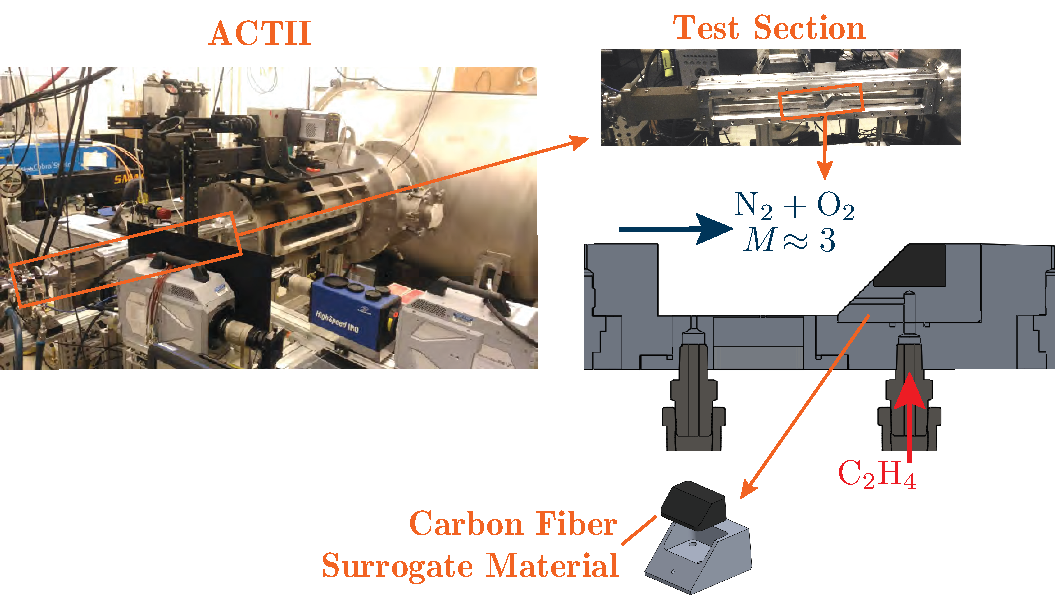
\includegraphics[width=0.9\textwidth]{Figures/actii-y0-setup.pdf}}
%  %\onslide*<2>{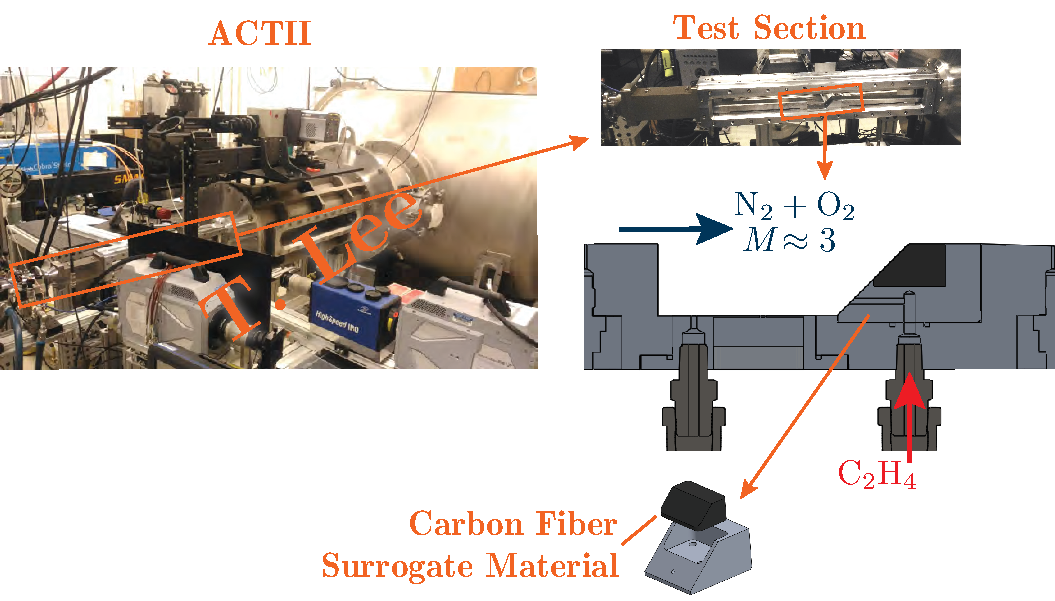
\includegraphics[width=0.9\textwidth]{Figures/actii-y0-setup-NAMES.pdf}}
%  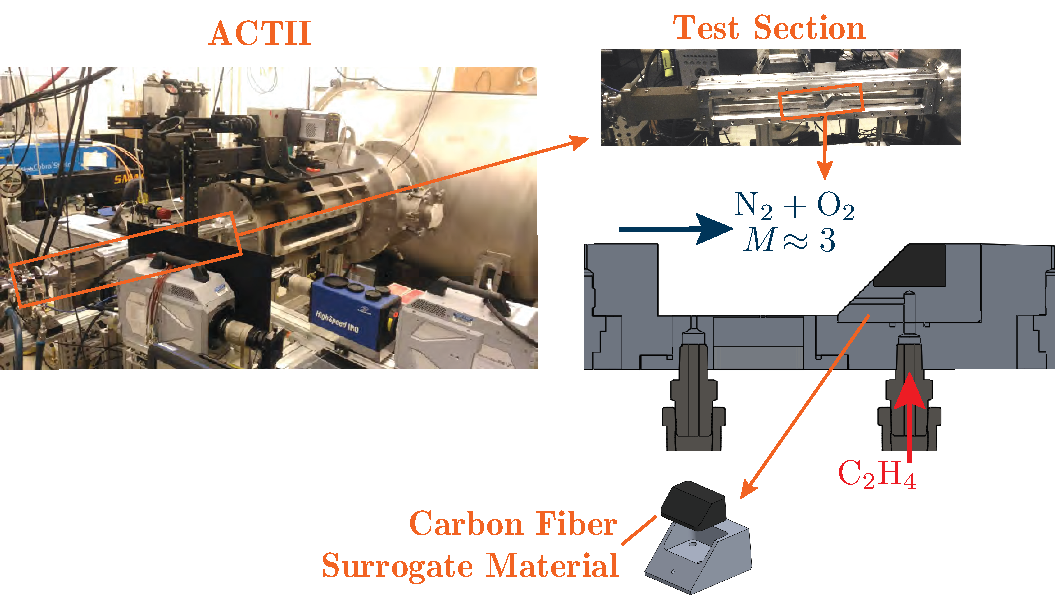
\includegraphics[width=0.9\textwidth]{Figures/actii-y0-setup.pdf}
%  \end{center}
%  
%  \end{frame}
%  
%  %======================================================================
% 
%\begin{frame}\frametitle{Experimental Setup - Unstart in a Free-Jet Scramjet}
%
%   \vspace{10pt}
%	\begin{minipage}{0.59\textwidth}
%	  \begin{itemize}
%	    \item ACTII Experimental facility
%	    \item Mach 4.5 nozzle
%	    \item Varying inlet contraction ratio
%	    \item Low ($CO_2$) and high ($O_2/N_2/C_2H_4$) enthalpy runs
%	    \item Mass injection or combustion induced unstart
%	  \end{itemize}
%
%	  \vspace{-10pt}
%	  	\begin{figure}
%	  	\centering
%	  	%\includegraphics[height=1.75in]{Figures/ACTII.pdf}
%	  		\includegraphics[height=1.6in]{Figures/ACTII_testChamber.pdf}
%	  	\end{figure}
%
%	\end{minipage}
%	\begin{minipage}{0.39\textwidth}
%	\begin{figure}
%		%\vspace{12pt}
%		\centering
%	  \includegraphics[height=1.4in]{Figures/scramjetModel.pdf}
%	\end{figure}
%	
%		\begin{singlespace} 
%		\tiny Baccarella, Experimental Study of Flow Choking and Inlet Unstart in an Axisymmetric Model Scramjet. 2018. University of Illinois.
%		\end{singlespace}
%	\end{minipage}
%
%
%\end{frame}
%
%\begin{frame}\frametitle{Modeling Timeline Y0/Y1}
%\cPI {Goal:} \PCtwo~simulations provide Y1 prediction and development milestones for \ceesdcode
%
%\hfill
%
%\cPI{Y0 Target:} October 2020
%\begin{itemize}
%	\item Low enthalpy, unstart by mass injection
%	\begin{itemize}
%	\item $CO_2$ flow, $N_2$ injection
%	\item 4 port, supersonic injection
%	\end{itemize}
%\end{itemize}
%
%\cPI{Y1 Target:} Winter 2020/Spring 2021
%\begin{itemize}
%\item High enthalpy, unstart by mass injection
%\begin{itemize}
%\item 16 port injector, air injection
%\end{itemize}
%\item High enthalpy, unstart by combustion
%\begin{itemize}
%\item 16 port injector, $C_2H_4$ injection, auto-ignition
%\end{itemize}
%\end{itemize}
%
%
%\end{frame}
%%======================================================================
%
%\begin{frame}\frametitle{Y1 Prediction Targets}
%
%\begin{minipage}{0.49\textwidth}
%\cPI{Qualitative}
%\begin{itemize}
%\item Unstart Go/No-Go
%\item PLRS comparison
%\end{itemize}
%
%\cPI{Quantitative}
%\begin{itemize}
%\item Scramjet model pressure
%\item Shock/pressure oscillation frequency
%\end{itemize}
%\end{minipage}
%\begin{minipage}{0.49\textwidth}
%\centering
%\includegraphics[height=1.7in]{Figures/Go-NoGo.pdf}
%\end{minipage}
%
%\centering
%\includegraphics[width=.7\textwidth]{Figures/PLRS-1.pdf}
%
%\end{frame}
%
%
%
%%======================================================================
%
%
%\begin{frame}\frametitle{Numerical Setup - PlasCom2}
%
%\vspace{10pt}
%	\begin{minipage}{0.59\textwidth}
%	  \begin{itemize}
%	    \item Mesh generation tool based on CAD
%	    \item Nine overset meshes
%	    \item Variable resolution in nozzle, scramjet model
% 	    \begin{itemize}
%			\item HalfX - $9.8 M$
%			\item OneX - $69 M$
%			\item OneX+ - $170 M$
%			\item OneX++ - $973 M$
% 	    \end{itemize}
%	    \item OneX resolution sufficient to resolve inlet shocks and nozzle boundary layer
%	    \item Increase scramjet interior resolution to capture turbulence leading to unstart
%	  \end{itemize}
%	\end{minipage}
%	\begin{minipage}{0.39\textwidth}
%	\begin{figure}
%
%		\centering
%	  \includegraphics[width=2in]{Figures/CAD.pdf}
%	\end{figure}
%	\vspace{-15pt}
%	\begin{figure}
%		\centering
% 		\includegraphics[width=1.4in]{Figures/inletMesh.pdf}
%	\end{figure}
%	\end{minipage}
%	\begin{figure}
%	\centering
%	\includegraphics[height=.9in]{Figures/meshPieces.pdf}
%	\end{figure}
%
%\end{frame}
%
%\begin{frame}
%physics (eqns)
%eos (model closure)
%boundary conditions (numerical closure)
%initialization
%sample results
%\end{frame}
%
%%\begin{frame}\frametitle{HalfX vs OneX}
%%
%%  \cPI{Y0 flowthrough}
%%  \begin{itemize}
%%    \item Qualitative comparison, $2.22x10^{-3} s$
%%    \item Constant gamma EOS
%%	\end{itemize}
%%
%%  \begin{figure}
%%  \centering
%%    \includegraphics[height=2.in]{figures/halfx_v_onex_M.pdf}
%%  \end{figure}
%%\end{frame}
%
%
%
%\begin{frame}\frametitle{Sample Scramjet Interior Pressure?}
%
%   \vspace{10pt}
%	\begin{figure}
%		%\vspace{12pt}
%		\centering
%	  \includegraphics[height=1.4in]{Figures/scramjetPressure.pdf}
%	\end{figure}
%
%	 \begin{itemize}
%	  \item Favorable comparison for initial shock structures
%	  \item Under-resolved BL structures?
%	 \end{itemize}
%	 
%\end{frame}
%	 
%
%       
%	 
%
%
%
%
%
%
%%======================================================================
%\begin{frame}\frametitle{}
%
%\vspace*{0.2in}
%
%\begin{center}
%
%\includegraphics[width=0.5\textwidth]{Figures/ceesd-logo-2.pdf}
%
%\vspace*{0.35in}
%\cPI{\huge Questions?}
%
%\vspace*{0.5in}
%\begin{minipage}{0.8\textwidth}
%This material is based in part upon work supported by the Department of Energy, National Nuclear Security Administration, under Award Number \textit{TBD}. 
%\end{minipage}
%
%\end{center}
%
%
%\end{frame}
%%======================================================================
%
% 

\end{document}


